\Chapter{CONVOLUTIONAL NEURAL NETWORK WITH COMMENTS AND SOURCE CODE}\label{sec:Theme3}

% TOTAL = 15 pages

%	./train.py --enable_word_embeddings true --num_epochs 6 --dev_sample_percentage 0.01 --positive_train=$pos --negative_train=$neg
%	
%	Used for the 3-Folds
%
% ./word2vec -train ../../tokenized-concordia-no-comment.txt -output concordia-bin-64.bin -size 100 -window 5 -sample 1e-4 -negative 5 -hs 0 -binary 1 -cbow 1 -iter 3

\section{Convolutional Neural Network}

%1 page

Several machine learners were tested with TEDIOUS, using source code metrics as training features. Results were promising but the approach asked for a lot of preparation work: building the XML representation of the Java code, pattern matching between comments from the dataset and the source code, extracting the source code metrics, extracting the warning raised by static analysis tools and feature preprocessing. These additional steps take time and knowledge of the whole process. Consequently, we wanted to try a novel approach, easier and faster to set up. We decided to test a Convolutional Neural Network (CNN) with Natural Language Processing (NLP) directly on the Java source code of software projects.

The idea of using a CNN was inspired by a paper written by \citet{kim2014convolutional}. He used a CNN for sentence-level classification tasks and showed that you can achieve excellent performance results with little parameter calibration. He tested his model on several benchmarks. Similar work has been pursued concerning sentiment analysis of short texts \citep{dos2014deep}. More specifically, they analyzed Twitter messages and movie reviews, and tried to classify them as being of positive or negative sentiment. Our idea is similar to these studies, we plan to use a CNN to classify comments and/or methods using the source code directly instead of features, linking them to technical debt or not.

Typically, convolutional neural networks were employed for image classification \citep{krizhevsky2012imagenet}, however, as mentioned previously, this type of neural network has been used recently combined with NLP. To describe CNN in further details, we can think of a convolution as a window sliding across a whole matrix, acting as a filter. For images, this matrix contains pixels, for words and sentences, it contains word vectors (word embeddings). In image classification, filters slide over local batches, in NLP, they slide over entire rows since a row is typically a single word embedded into a row matrix of the size of the embedding dimension. To implement a CNN, you just have to add several layers of these convolutions, where each of these layers have a specific task and act as different filters. CNNs are very fast and efficient in terms of representation, which means they give good representations without needing the whole vocabulary of a dataset.

The main purpose of this study was to explain, test and analysis TEDIOUS, our machine learning approach using source code features. The next sections will describe the other approach using a CNN, but at a more general level than for TEDIOUS since we are still at a preliminary stage. Since some steps from Chapter 3 are replicated in our CNN approach, they will be explained rapidly in order to avoid redundancy. However, we still judged interesting to present the initial results of this new promising method.

\section{The Approach}

%1 page

This section will describe the steps followed to design this new approach, a convolutional neural network combined with natural language processing to identify technical debts to self-admit. Additional information will be shared on the characteristics of this machine learner and how it works. Like TEDIOUS, this approach works at method-level since it is granularity at which we are most likely to detect TD \citep{PotdarS14}. In other terms, this approach is able to detect if a technical debt is contained in a method or not.

\begin{figure}[t]
	\centering
	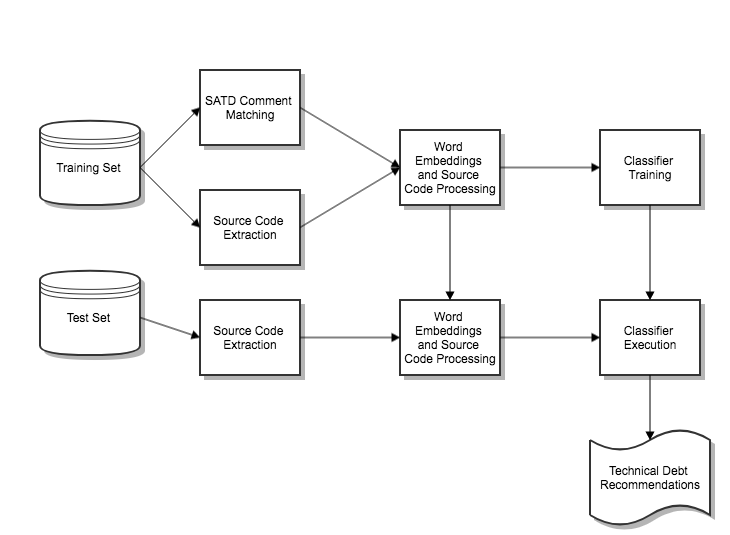
\includegraphics[width=\linewidth]{figs/CNN.png}
	\caption{Proposed approach for recommending SATD with a CNN.}
	\label{fig:CNN}
	\vspace{-4mm}
\end{figure}

As shown in Figure \ref{fig:CNN}, two datasets are required to build our model: the training and test set. The training set contains labeled data, which is source code where SATD are known. The test set contains unlabeled data, which can be any source code where we want to recommend where technical debts should be admitted. The presence and location of TDs are unknown in the test set.

For the training set, various combinations of source code and comments, labeled as containing a SATD or not, are extracted: source code comments only, source code with comments, source code without comments and source code partially with comments. It is essential to have this classification because the CNN is based on supervised learning. Pattern matching using comments from the dataset of \citet{maldonado17} is employed to classify the methods and comments.

Once all the source code is extracted and classified, some preprocessing has to be done. The source code is tokenized, the purpose being to demarcate and transform the source code into a string of word tokens. The comments specifically are cleaned up to remove extra spaces, non-ASCI characters, upper case letters, etc. Once the source code is preprocessed, word embeddings is performed, which means strings of tokens are transformed into vectors of numerical values using word2vec tool \citep{word2vec}. With the source code preprocessed and the oracle built, the model can be trained with the CNN.

In parallel, the test set is prepared. The same combinations of source code and comments are extracted, but SATD matching is not required because the data is unlabeled and we want to predict the presence of technical debts. The matching of SATDs is only required for the oracle to train models. The same preprocessing and word embeddings are applied on the dataset. With the previously trained model and the test set, predictions can be made in order to recommend when to self-admit technical debts.

An overview of the process was described in this section, but more details will be shared in the next ones. We will discuss the source code and its nature, how we identified the SATD, how we performed word embeddings and the process to train and apply the models generated by the CNN.

\subsection{Source Code}

% 1 page

The main difference between TEDIOUS and this new approach is the nature of the training features. For TEDIOUS, source code metrics and warnings were used. For the CNN, we use the source code itself, transformed into word vectors. The same process was performed as before to extract the source code, an XML representation of the Java source code was generated using the srcML tool \citep{Collard2013}. SATD comments from the dataset of \citet{MaldonadoNLP} were linked to their respective methods in order to classify them as containing a technical debt or not, to build the oracle. The same rules were followed, as explained in section 3.1.1. Once the XML representation is obtained, the different dataset combinations can be generated.

The first combination is the \textit{source code comments only}. They are extracted from the dataset of comments provided by \citet{maldonado17}. Comments can be encountered under different natures: single line, multiple lines or block. It is important to specify that not only design debts were retained but all of them, namely: defect, design, documentation, implementation and test. We decided to use as many SATD-methods as possible in order to have the best chances at getting good predictions results. By using different types of technical debts, we decrease the unbalance of the dataset by adding more positive examples.

The second combination is the \textit{source code with comments} where the complete XML representation of the source code is used. The third combination is the \textit{source code without comments} where the XML representation is parsed to remove comments. The fourth combination is the \textit{source code partially with comments}, which means only comments related to SATD are removed. The reason behind this removal is to be sure to avoid the CNN model being a self-prophecy. For these three datasets, only design and implementation TDs are retained, to be more in line with the dataset used by TEDIOUS. The details of the process behind the extraction of each combination will be explained in the Source Code Preprocessing section.

\subsection{Identification of Self-Admitted Technical Debt}

% 0.5 page

Like TEDIOUS, the purpose of this approach is not to propose a new way to detect SATD using information from comments. However, will still needed a classified dataset in order to train our CNN model. We used the dataset of \citet{maldonado17}, which contains a classification of 10 open source projects, where methods are tagged as containing a technical debt or not. Various types of TDs are considered, depending on the source code combination. The dataset reports SATD at file-level instead of method-level, consequently, some preprocessing had to be performed. With pattern matching, SATD comments were tagged to their related methods.

\subsection{Source Code Preprocessing and Word Embeddings}

% 1 page

The source code is extracted in a XML format, which is not quite compatible for the machine learner to train on. The files have to be tokenized. Instead of using standard coding lexicon (conditional statements, variables types and names, parameters declaration) and separators (brackets, parentheses, spaces) directly in our dataset, demarcations are added (\textit{i.e. begin\_type, end\_type}) to transform the structure into series of word tokens. For comments, strings are normalized: extra spaces are removed, upper cases are transformed to lower cases, non-ASCI are removed as well as new lines. Also, if a comment is matched with a SATD pattern, it will be printed as:

\textsc{comment\_begin\_satd    comment-normalized-text    comment\_end\_satd}

This step is essential to build the oracle and the dataset partially with comments. By explicitly defining comments tagged as SATD in this format, it is easy to parse the tokenized dataset in order to remove them. Comments are linked to their respective method, so a method linked to a SATD comment will also be tagged as SATD. By tokenizing the source code, it is also easier to remove the comments globally, if necessary. Transforming the source code into tokens also acts as a normalization process, which will make the word embedding process more efficient.

Word embeddings is the process of transforming words and phrases from the dataset into vectors of real number. Word2vec models were used to generate word embeddings. The vector dimension we used is 100, we tried to have a balance between a proper representation of words and processing time. A new word embedding was generated for each source code combination since they are all different in some ways.

Finally, the methods extracted are all tagged as positive or negative examples. In order for the CNN to be trained and tested, these methods have to be divided in 4 basic files: \textsc{positive-train}, \textsc{negative-train}, \textsc{positive-test} and \textsc{negative-train}. Each fold of the cross validation contains these 4 files, consequently, for a 10-fold cross validation, 40 files are required. Instead of using an additional feature to classify each method in a single file, the files act as classifiers. Here is a detailed definition of each file, considering a 10-fold cross validation:

\begin{itemize}
	\item \textit{Positive-Train}: Training set containing SATD methods (90\% of all positive examples)
	\item \textit{Negative-Train}: Training set containing non-SATD methods (90\% of all negative examples)
	\item \textit{Positive-Test}: Testing set containing SATD methods (10\% of all positive examples)
	\item \textit{Negative-Test}: Testing set containing non-SATD methods (10\% of all negative examples)
\end{itemize}

\subsection{Building and Applying CNN}

% 2 page

\begin{figure}[t]
	\centering
	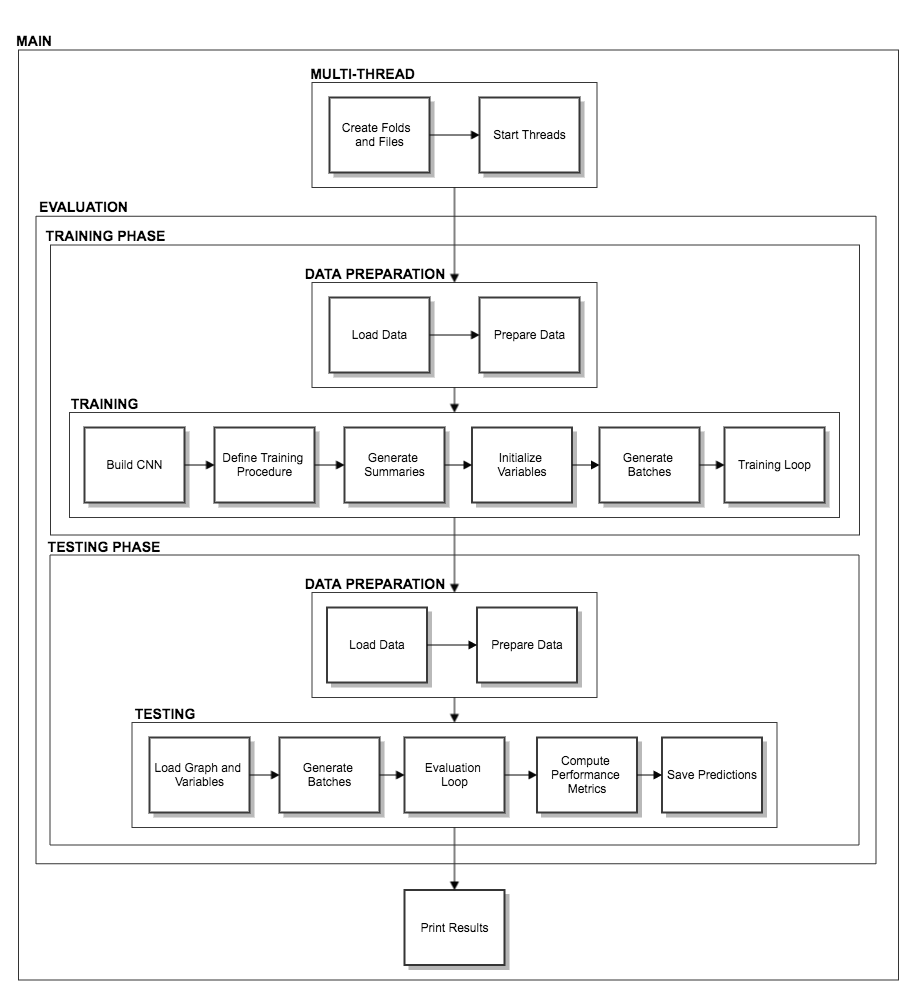
\includegraphics[width=\linewidth]{figs/CNNProcess.png}
	\caption{Process for building and applying a CNN.}
	\label{fig:CNNProcess}
	\vspace{-4mm}
\end{figure}

So far, we extracted source code from various projects, with or without comments, we identified SATD methods, we preprocessed the dataset and performed a word embedding. The only step remaining is building and applying the convolutional neural network. Four sets are required, as described in the previous section: two sets for training, one containing SATD methods and the other not, and two sets for testing, one of positive and the other of negative examples. The sets contain the tokenized source code of the nine studied projects.

Figure \ref{fig:CNNProcess} provides an overview of the CNN process. To increase the training speed and to benefit as much as possible from the processing power available, several threads are created. One thread is started for each fold, using a pair of previously generated training files. Up to five threads can be processed at the same time. The next actions are all performed simultaneously on each thread, until we have models trained for all folds. 

The evaluation process consists of two main phases: the training and the testing phase. In the former, some data preparation is required: load the two training sets, build the vocabulary, shuffle, and split the dataset in a training and development set. The development set is used to tune parameters of the CNN and to prevent it from over-fitting. Afterwards, the CNN is built using user-defined parameters and default values. In our case, mainly the default configuration is considered. The training procedure is defined and summaries are generated for: loss, accuracy, train, development and model. Then, variables are initialized, such as embedding vectors, and training batches generated. Finally, a training loop is executed where a training and evaluation step are repeated. The trained model is saved multiple times during the loop and the last one is used for the testing. 

The testing phase can start once the training is finished. Data preparation is also required for this step: load the two testing sets and map them into the vocabulary. Afterwards, the meta graph and the variables from the model previously saved are loaded. Testing batches are generated and tensors we want to evaluate are determined. We can then start the testing loop where predictions are made. Once over, performance metrics can be computed,  namely: accuracy, recall, precision, specificity and $F_1$. These metrics are saved in a different file from the predictions made on each method. The final step consists of combining the performance metrics of all models for further analysis.

\section{Study Definition}

% 0.5 page

The goal of this new approach is to assess the prediction performance of a convolutional neural network in recommending technical debts to self-admit. The focus is the same as for TEDIOUS, enhancing the source code quality by keeping track of TDs. The perspective is to be able to suggest to developers, more accurately than with TEDIOUS, when to admit technical debts. We aim to address four research questions:

\begin{itemize}
	\item \textbf{RQ1}: How does a CNN work for recommending SATD with source code comments only?
	\item \textbf{RQ2}: How does a CNN work for recommending SATD with source code  with comments?
	\item \textbf{RQ3}: How does a CNN work for recommending SATD with source code without comments?
	\item \textbf{RQ4}: How does a CNN work for recommending SATD with source code partially with comments?
\end{itemize}

\subsection{Dataset}

% 1.5 page

\begin{landscape}
	\begin{table*}[t]
		\caption{Characteristics of the studied projects.}
		\label{tab:projects}
		\centering
		\begin{adjustbox}{center}
			\begin{tabular}{l r | r r r r | r | r r | r}
				\hline
				\multirow{2}{*}{Project} & \multirow{2}{*}{Release} &\multicolumn{4}{c|}{Number of} &\multicolumn{1}{c|}{Number of Comments}
				&\multicolumn{2}{c|}{Number of Design SATD} & \% of Methods\\
				&& Files& Classes& Methods& Comments                      & $\in$ Methods& $\notin$ Methods & $\in$ Methods & with design SATD\\
				\hline
				Ant&1.7.0 & 1,113 & 1,575 & 11,052 & 20,325               & 13,359        &  1 & 57 & 0.5\% \\
				ArgoUML&0.34& 1,922 & 2,579 & 14,346 & 64,393       &  17,722       & 203 & 425  & 2\%\\
				Columba&1.4& 1,549 & 1,884 & 7,035 & 33,415           & 10,305        & 8 & 418 & 5\%  \\
				Hibernate&3.3.2 GA & 2,129 & 2,529 & 17,405 & 15,901 & 9,073        & 21  &  377  &  2\%\\
				jEdit & 4.2 & 394 & 889 & 4,785 & 15,468                     &10,894         & 6  & 77  & 2\% \\
				jFreeChart&1.0.19 & 1,017 & 1,091 & 10,343 & 22,827  & 15,412       &  4  & 1,881  & 18\%\\
				jMeter&2.1& 1,048 & 1,328 & 8,680 & 19,721                &  12,672      & 95 &  424 & 5\%  \\
				jRuby&1.4.0 & 970 & 2,063 & 14,163 & 10,599               & 7,809        & 16   & 275  &  2\%\\
				Squirrel&3.0.3 & 2,325 & 4,123 & 16,648 & 25,216         & 15,574      &35  & 173  & 1\%\\
				\hline
			\end{tabular}
		\end{adjustbox}
		\vspace{-4mm}
	\end{table*}
\end{landscape}

To evaluate this new approach, the same dataset was used as in TEDIOUS \citep{maldonado17}. The methods are already classified as SATD or not, and Table \ref{tab:projects} summarizes the characteristics of all studied projects. Various information describe the content and nature of each project. This table was already presented in Section 3.2.1. However, a brief overview is still necessary to reiterate important facts. 

There are some disparities between the results we obtained when analyzing the studies and what \citet{maldonado17} obtained. However, this does not really represent an issue since many of these differences concern classes while our CNN approach is method-level based, like TEDIOUS. This aspect is also important since we clearly see a prevalence of method-related rather than class-related SATD. Out of all methods in a project, only a very small amount contains a technical debt, making the dataset highly unbalanced. As we will discuss in the analysis of results, the lower the amount of technical debts in a system, the lower the prediction performance. Since the dataset from \citet{maldonado17} classified classes instead of methods, we performed pattern matching between known SATD comments and comments attached to methods in the dataset.

\subsection{Analysis Method}

% 2 pages

For \textbf{RQ1}, we want to know how a convolutional neural network with source code comments only work for recommending SATD within-project. We also want to compare the results with the within-project predictions of TEDIOUS. A 10-fold cross validation was performed on each project, like for TEDIOUS, and the performance values are averaged over the 10 iterations. The same process is followed for \textbf{RQ2}, \textbf{RQ3} and \textbf{RQ4}.

Standard performance metrics on the SATD category were computed to evaluate our automated classification approach: precision, recall, $F_1$ score and accuracy. Precision is the percentage of relevant instances of methods predicted as SATD among all retrieved instances. Recall is the percentage of relevant instances of SATD methods that have been retrieved over all relevant instances. $F_1$ score is the harmonic mean between precision and recall. Accuracy is the total number of methods correctly predicted, whether it is SATD-related or not, among all analyzed methods. 

Unfortunately, metrics such as MCC, ROC and importance of features were not computed for this approach. However, we still have enough information to evaluate and compare each approach. The downside is that it will be more difficult to take into account the effect of chance on predictions. Overall, what we look for in a good classifier is a balance between precision and recall while aiming for the highest $F_1$ score. We want to detect as many technical debts as possible while being correct in our predictions.

\section{Study Results}

This section reports the results obtained using various combinations of source code. Performance metrics are presented in tables and further analysis is provided textually, discussing the metrics and comparing them with TEDIOUS.

\subsection{Source Code Comments Only}

%1.5 pages 

Table \ref{tab:commentsonly} reports the within-project performance results of a 10-fold cross validation on each system using our convolutional neural network and source code comments only. We computed the average for the 10 folds of each system and for the complete dataset. Since we already had the comments preprocessed for TEDIOUS, this dataset was a good start to test our CNN approach.

\begin{table}[t]
	\caption{Within-project prediction: results of CNN for each system using source code comments only}
	\label{tab:commentsonly}
	\centering\scriptsize
	\resizebox{\linewidth}{!}{
		
		\begin{tabular}{lrrrr}
			%\hline
			\multicolumn{5}{c}{ \textbf{Source Code Comments Only}}\\
			\hline
			\textbf{System} & \textbf{Pr} & \textbf{Rc }&\textbf{F$_{1}$} &\textbf{Acc}\\
			\hline
			Ant & 93.33 & 10.77 & 19.31 & 97.02\\
			ArgoUML &91.21& 90.94 & 91.07 & 97.24\\
			Columba & 97.12 & 71.05 & 82.07 & 99.08\\
			Hibernate & 95.29 & 73.19 & 82.79 & 95.12\\
			jEdit & 82.95 & 29.32 & 43.32 & 98.09\\
			jFreeChart & 100.00 & 69.38 & 81.92 & 98.50\\
			jMeter & 95.25 & 75.95 & 84.51 & 98.71\\
			jRuby & 96.14 & 87.17 & 91.43 & 97.89\\
			Squirrel & 95.81 & 65.59 & 77.87 & 98.51\\
			\textbf{Total} & \textbf{93.63} & \textbf{76.17} & \textbf{84.00} & \textbf{97.99}\\
			\hline
		\end{tabular}
	}
	\vspace{-3mm}
\end{table}

Two systems perform significantly worse than the others, namely \textsc{Ant} and \textsc{jEdit}. We face the same problem as in TEDIOUS, where the very low percentage of SATD methods (\textsc{Ant} has 0.5\% and \textsc{jEdit} has 2\%) in some systems directly affects the performance of the CNN. \textsc{Ant} has a precision of 93.33\%, recall of 10.77\% and $F_1$ score of 19.31\%. \textsc{jEdit} is a little better, it has a precision of 82.95\%, recall of 29.32\% and $F_1$ score of 43.32\%. However, if we compare with results from TEDIOUS, we notice a significant improvement in precision while maintaining a similar recall for these two systems.

As for the other systems, the precision is $> 91\%$, the recall is $> 65\%$ and the $F_1$ $> 77\%$. Differently from TEDIOUS where the best results were obtained with \textsc{jFreeChart}, \textsc{ArgoUML} is the system where the CNN performed the best (precision 91.21\%, recall 90.94\% and $F_1$ 91.07\%). \textsc{jFreeChart} still obtained the best precision (100\%) but other projects such as \textsc{jRuby} or \textsc{jMeter} provided more balanced performance values. We have to be careful when comparing results in this scenario because all types of technical debts were considered whereas TEDIOUS only analyzed design debts. 

However, on first look, it seems that the CNN approach using source code is an improvement of TEDIOUS using source code features. The total average precision, recall and $F_1$ score is even higher than the best system using TEDIOUS. Further testing is needed to provide a better understanding of the performance of the CNN, which will be accomplished in the next sections.

% \Desktop\CNN-results.csv
% \noiseux1523\cnn-text-classification-tf-w2v 
%		dans \encoded-comment-files pour le data
%		dans \run-all.sh pour le process

\subsection{Source Code With Comments}

%1.5 pages

Using source code comments only is an interesting first step to train a convolutional neural network to predict technical debts, especially if we aim at addressing the issue of self-admitted technical debts. However, it would also be interesting to see how well a CNN can perform using the entirety of a project's source code, code and comments included. We experimented with such a dataset and obtained the results reported in Table \ref{tab:comments} for a within project 10-fold cross validation.

\begin{table}[t]
	\caption{Within-project prediction: results of CNN for each system using source code with comments}
	\label{tab:comments}
	\centering\scriptsize
	\resizebox{\linewidth}{!}{
		
		\begin{tabular}{lrrrr}
			%\hline
			\multicolumn{5}{c}{ \textbf{Source Code With Comments}}\\
			\hline
			\textbf{System} & \textbf{Pr} & \textbf{Rc }&\textbf{F$_{1}$} &\textbf{Acc}\\
			\hline
			Ant & 95.24 & 66.67 & 78.43 & 99.81\\
			ArgoUML &97.32& 87.88 & 92.36 & 98.84\\
			Columba & 93.62 & 80.00 & 86.27 & 99.66\\
			Hibernate & 95.61 & 89.71 & 92.56 & 99.72\\
			jEdit & 100.00 & 21.00 & 34.71 & 98.25\\
			jFreeChart & 97.73 & 90.72 & 94.09 & 99.72\\
			jMeter & 96.45 & 82.61 & 88.99 & 99.45\\
			jRuby & 94.35 & 76.80 & 84.67 & 98.70\\
			Squirrel & 98.57 & 85.19 & 91.39 & 99.92\\
			\textbf{Total} & \textbf{96.38} & \textbf{82.40} & \textbf{88.84} & \textbf{99.44}\\
			\hline
		\end{tabular}
	}
	\vspace{-3mm}
\end{table}

Again, the worst results were obtained for \textsc{Ant} and \textsc{jEdit}. However, compared to source code comments only, \textsc{Ant} improved its precision by $+ 1.91\%$, recall by $+ 55.90\%$ and $F_1$ by $+ 59.12$, and \textsc{jEdit} improved its precision to 100\% but suffered some losses in its recall and $F_1$ score. We notice that the unbalance of the dataset is still an issue for the CNN but these results are still better than what we obtained with TEDIOUS.

As for the other systems, the precision varies between $[93.62\%-98.57\%]$, the recall between $[76.80\%-90.72\%]$ and the $F_1$ score between $[84.67\%-94.09\%]$. Precision is generally slightly better and the recall gains a decent improvement compared to the source code comments only dataset. The best results were obtained with \textsc{jFreeChart} (precision $97.73\%$, recall $90.72\%$ and $F_1$ score $94.09\%$), like in TEDIOUS but not the previous dataset. This can be explained by the fact that we only used design and implementation debts, compared to all types of debt for source code comments only. Consequently, results with this dataset should normally be more similar to the results of TEDIOUS.

If we look at the average total performance values, there is an improvement compared to the source code comments only dataset: precision $+ 2.75\%$, recall $+ 6.23\%$ and $F_1$ $+ 4.84\%$. Consequently, using the whole source code is also an improvement compared to TEDIOUS, in a pretty significant manner. We just tested the best case scenario where we have as much information as possible to train on, however, we also want to know how well a CNN can perform on a less than ideal software project.

% \Desktop\stats-baseline-with comments.csv
% dans \yes-and-no pour le data
% dans \run-all.v2.sh pour le process

\subsection{Source Code Without Comments}

%1.5 pages

\begin{table}[t]
	\caption{Within-project prediction: results of CNN for each system using source code without comments}
	\label{tab:withoutcomments}
	\centering\scriptsize
	\resizebox{\linewidth}{!}{
		
		\begin{tabular}{lrrrr}
			%\hline
			\multicolumn{5}{c}{ \textbf{Source Code Without Comments}}\\
			\hline
			\textbf{System} & \textbf{Pr} & \textbf{Rc }&\textbf{F$_{1}$} &\textbf{Acc}\\
			\hline
			Ant & 50.00 & 1.67 & 3.23 & 99.48\\
			ArgoUML &89.78& 37.27 & 52.68 & 94.67\\
			Columba & 84.21 & 14.55 & 24.81 & 98.81\\
			Hibernate & 79.66 & 27.65 & 41.05 & 98.43\\
			jEdit & 72.73 & 24.00 & 36.09 & 98.11\\
			jFreeChart & 73.68 & 17.72 & 28.57 & 97.85\\
			jMeter & 83.61 & 22.17 & 35.05 & 97.77\\
			jRuby & 95.27 & 56.40 & 70.85 & 97.84\\
			Squirrel & 88.89 & 17.78 & 29.63 & 99.56\\
			\textbf{Total} & \textbf{88.18} & \textbf{33.68} & \textbf{48.75} & \textbf{98.12}\\
			\hline
		\end{tabular}
	}
	\vspace{-3mm}
\end{table}

We trained our convolutional neural network on source code comments only and on source code in addition to comments. We obtained promising results, but we want know how well our machine learner can work with less training information. We generated another dataset, this time only containing the source code of the studied projects, eliminating the comments. We built such a dataset to replicate the worst case where a software project is lacking comments and to remove SATD comments related to their respective methods. Table \ref{tab:withoutcomments} reports the performance results for each system using a 10-fold cross validation and source code without comments as the training set.

\textsc{Ant} is still the system where the CNN performs the worst (precision $50.00\%$, recall $1.67\%$ and $F_1$ $3.23\%$), in line with every other experiment we performed so far. However, \textsc{jEdit} is performing decently compared to previously and, surprisingly, \textsc{jFreeChart} is average even though it contains the most design debts. It seems the unbalance of the dataset does not correlate as much with the results since \textsc{jRuby} obtains the best performance (precision 95.27\%, recall 56.40\% and $F_1$ 70.85\%) only with 2\% of methods with design SATD.

As for the other systems, performance metrics all decreased compared to the last two datasets, especially the recall. If we compare the total average, at the most, precision decreases of $- 8.21\%$, recall of $-48.72$ and $F_1$ of $-40.09\%$. Compared to TEDIOUS, the precision is generally better but the recall rate worst. It would be difficult, with the available information, to determine which machine learner performs better between TEDIOUS and CNN with source code without comments. However, it is safe to say that they are at least similar performance wise, with TEDIOUS providing better recall and the CNN better precision.

Overall, it is obvious that removing comments from the dataset impacts the performance of the CNN at all levels. It is clear that they represent an important piece of information for the machine learner to train on and should be kept in the dataset. We also notice that not only the amount of technical debts in a system is important to obtain good performance, but the nature of technical debts and the content of the source code as well. When removing comments, we observed that different systems would perform better than previously and other worst, despite having the same amount of SATD-methods. Knowing the importance of comments, one more experiment would be interesting to complete to better understand why.

% \Desktop\stats-baseline-with-no-comments.csv
% dans \yes-and-no pour le data
% dans \run-all.v2.sh pour le process

\subsection{Source Code Partially With Comments}

%1.5 pages

So far, the best results were obtained with a dataset consisting of source code with comments. When removing all comments, we observed a significant loss in recall, and a modest one in precision. We now want to test an intermediate dataset where we keep all comments except the SATD comments manually analyzed by \citet{maldonado17}. The main reason behind the generation of this new dataset is to quantify the impact of these specific comments on the prediction performance and to know if they act as a self-prophecy. In other terms, we want to know how well our convolutional neural network can predict technical debts in methods if we remove comments self-admitting them. Table \ref{tab:partialcomments} reports the performance results for each system using a 10-fold cross validation and source code partially with comments.

\textbf{AJOUTER LA TABLE CROSS PROJECT DE GIULIO. LES COMMENTS LIES AUX METHODS SATD SONT ENLEVES POUR EVITER SELF PROPHECY}

\begin{table}[t]
	\caption{Within-project prediction: results of CNN for each system using source code partially with comments}
	\label{tab:partialcomments}
	\centering\scriptsize
	\resizebox{\linewidth}{!}{
		
		\begin{tabular}{lrrrr}
			%\hline
			\multicolumn{5}{c}{ \textbf{Source Code Partially With Comments}}\\
			\hline
			\textbf{System} & \textbf{Pr} & \textbf{Rc }&\textbf{F$_{1}$} &\textbf{Acc}\\
			\hline
			Ant & 96.88 & 51.67 & 67.39 & 99.74\\
			ArgoUML &95.40& 60.81 & 74.28 & 96.65\\
			Columba & 100.00 & 39.09 & 56.21 & 99.18\\
			Hibernate & 87.68 & 54.41 & 67.15 & 98.95\\
			jEdit & 100.00 & 40.00 & 57.14 & 98.67\\
			jFreeChart & 93.68 & 68.78 & 79.32 & 99.13\\
			jMeter & 97.46 & 50.00 & 66.09 & 98.61\\
			jRuby & 97.44 & 68.60 & 80.52 & 98.45\\
			Squirrel & 87.23 & 45.56 & 59.85 & 99.68\\
			\textbf{Total} & \textbf{94.84} & \textbf{58.83} & \textbf{72.61} & \textbf{98.82}\\
			\hline
		\end{tabular}
	}
	\vspace{-3mm}
\end{table}

% \Desktop\stats-baseline-no-manually-tagged-comments.csv
% dans \yes-and-no pour le data
% dans \run-all.v2.sh pour le process

All systems perform decently well and previously problematic ones, such as \textsc{Ant} and \textsc{jEdit}, are not outsiders anymore. The precision varies between $[87.23\%-100.00\%]$, the recall between $[39.09\%-68.78\%]$ and the $F_1$ score between $[56.21\%-80.52\%]$. In other terms, the CNN is able to predict at least half of the technical debts in a system with a very high precision. 

Compared to the dataset with all comments where results seemed somewhat dependent on the system, this one provides more balanced but weaker overall results. However, there is a net improvement compared to the dataset without comments. In fact, source code partially with comments positions itself right between the previous two datasets with a precision of 94.84\%, recall of 58.83\% and $F_1$ score of 72.61\%. Compared to TEDIOUS, our CNN with source code partially with comments is also an improvement.

We observe that SATD comments have an important impact on the prediction performance. The amount of comments removed is very small compared to the total, however, the impact on performance is not negligible, mostly on recall. It seems like comments, especially SATD-related, are important features for our machine learner to train on. We observe this fact in the way each system position themselves compared to others, some will benefit from keeping SATD-related comments and others will not. In addition, performance metrics globally decrease when removing comments.


















